% Source: fixed PDF source-relative page 2 (printed page 307), Q21.
% Ellipse, axes, focus F, chord AB through F, midpoint P, line m, and vertical line l follow the source diagram.
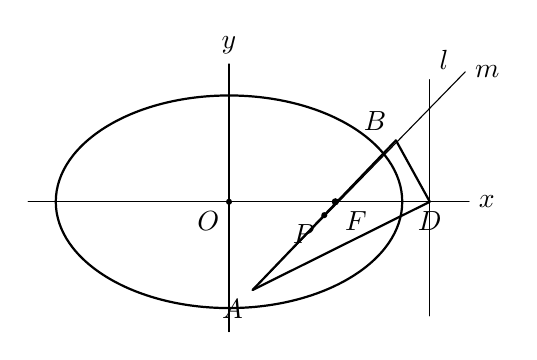
\begin{tikzpicture}[line cap=round,line join=round,>=stealth]
  \coordinate (O) at (0,0);
  \coordinate (F) at (1.35,0);
  \coordinate (A) at (0.3,-1.12);
  \coordinate (B) at (2.12,0.78);
  \coordinate (P) at (1.21,-0.17);
  \coordinate (D) at (2.55,0);
  \draw[thick] (0,0) ellipse (2.2 and 1.35);
  \draw[thin] (-2.55,0)--(3.05,0) node[right] {$x$};
  \draw[thin] (0,-1.65)--(0,1.75) node[above] {$y$};
  \draw[thick] (A)--(B);
  \draw[thick] (B)--(D) (A)--(D);
  \draw[thin] (A)--(3.0,1.65) node[right] {$m$};
  \draw[thin] (D)+ (0,-1.45) -- +(0,1.55) node[above right] {$l$};
  \fill (O) circle[radius=1.1pt];
  \fill (F) circle[radius=1.3pt];
  \fill (P) circle[radius=1.1pt];
  \node[below left] at (O) {$O$};
  \node[below right] at (F) {$F$};
  \node[below left] at (A) {$A$};
  \node[above left] at (B) {$B$};
  \node[below left] at (P) {$P$};
  \node[below] at (D) {$D$};
\end{tikzpicture}
